%%%%%%%%%%%%%%%%%%%%%%%%%%%%%%%%% METADADOS %%%%%%%%%%%%%%%%%%%%%%%%%%%%%%%%%%%%

\title[The shortened title]{Parallel GCC: Status and Expectations}
%\subtitle{The (optional) subtitle}

\author[Authors Name]{Giuliano Belinassi}

\institute[USP]{\textbf{GNU Cauldron 2019} \\ FLUSP \\ Computer Science Department \\ Institute of Mathematics and Statistics \\ University of São Paulo (USP)}
%\institute[USP]{\textbf{Orientador: Alfredo Goldman} \\ Departamentamento de Ciência da Computação \\ IME USP}

\date{August 15, 2019}

% Coloca a imagem no fundo da página de título
%\bgimage{\includegraphics[width=\paperwidth]{fundo_predios_e_grafo}}

% Logotipos no rodapé da página de título
%\logos{
%  \hfil\hfil\includegraphics[width=.1\textwidth]{usp-logo}\hfil%
%  \raisebox{-.0103\paperheight}{\includegraphics[height=.0932\paperheight]{interscity-logo}}\hfil%
%  \raisebox{-.033\paperheight}{\includegraphics[width=.07\textwidth,trim=0 230 0 0,clip]{ime-logo}}\hfil\hfil
%}
%
\logos{
  \hfil\hfil\includegraphics[width=.1\textwidth]{usp-logo}\hfil%
%  \raisebox{-.0103\paperheight}{\includegraphics[height=.0932\paperheight]{interscity-logo}}\hfil%
%  \raisebox{-.00517\paperheight}{
\includegraphics[height=.057\paperheight]{cnpq-logo}}\hfil%
  \raisebox{-.00517\paperheight}{
\includegraphics[height=.1\paperheight]{flusp-logo}}\hfil%
  \raisebox{-.02\paperheight}{
\includegraphics[height=.1035\paperheight]{capes-logo}}\hfil\hfil\strut%
%  \includegraphics[height=.044\paperheight]{fapesp-logo}\hfil\hfil
}

% Usado para criar o qrcode com o endereço da apresentação
%\presentationurl{http://interscity.org}

% Inclui o qrcode no sumário da apresentação
%\includeqrcodeintoc

% O slide de sumário pode ser dividido em colunas; o parâmetro
% determina após qual o número da seção fazer a quebra de coluna
% (use zero para uma coluna ou simplesmente omita este comando).
\toccolumns{4}


%%%%%%%%%%%%%%%%%%%%%%%%%%%%%%%%%%%%%%%%%%%%%%%%%%%%%%%%%%%%%%%%%%%%%%%%%%%%%%%%
%%%%%%%%%%%%%%%%%%%%%%%%%%%% INÍCIO DA APRESENTAÇÃO %%%%%%%%%%%%%%%%%%%%%%%%%%%%
%%%%%%%%%%%%%%%%%%%%%%%%%%%%%%%%%%%%%%%%%%%%%%%%%%%%%%%%%%%%%%%%%%%%%%%%%%%%%%%%

% É complicado colocar uma imagem de fundo, os logos das agências e
% o conteúdo "normal" do slide de título sem que as coisas fiquem
% bagunçadas, então definimos um comando para gerar o slide de título
\customtitlepage

% Slide com o qrcode
%\showqrcode


\begin{frame}[fragile]{Introduction}
    \begin{itemize}
        \item {\color{blue}{FLUSP}} -- Floss at USP
            \begin{itemize}
                \item Student Extension Group
                \item Aims to Contribute at FLOSS
                \item Projects we currently contribute: Linux Kernel, GCC, Git, Debian
                \item Promote {\color{blue}{Contribution Events}}, such as the KernelDevDay
            \end{itemize}
    \end{itemize}

    %\centering
    %
\includegraphics[scale=0.2]{flusp.png}
    %\\ This is Mr. FLUSP

\begin{figure}[ht]
\centering
  \begin{subfigure}[b]{0.49\textwidth}
 	
\includegraphics[height=0.4\paperheight]{flusp.png}
  \end{subfigure}
  \begin{subfigure}[b]{0.49\textwidth}
 	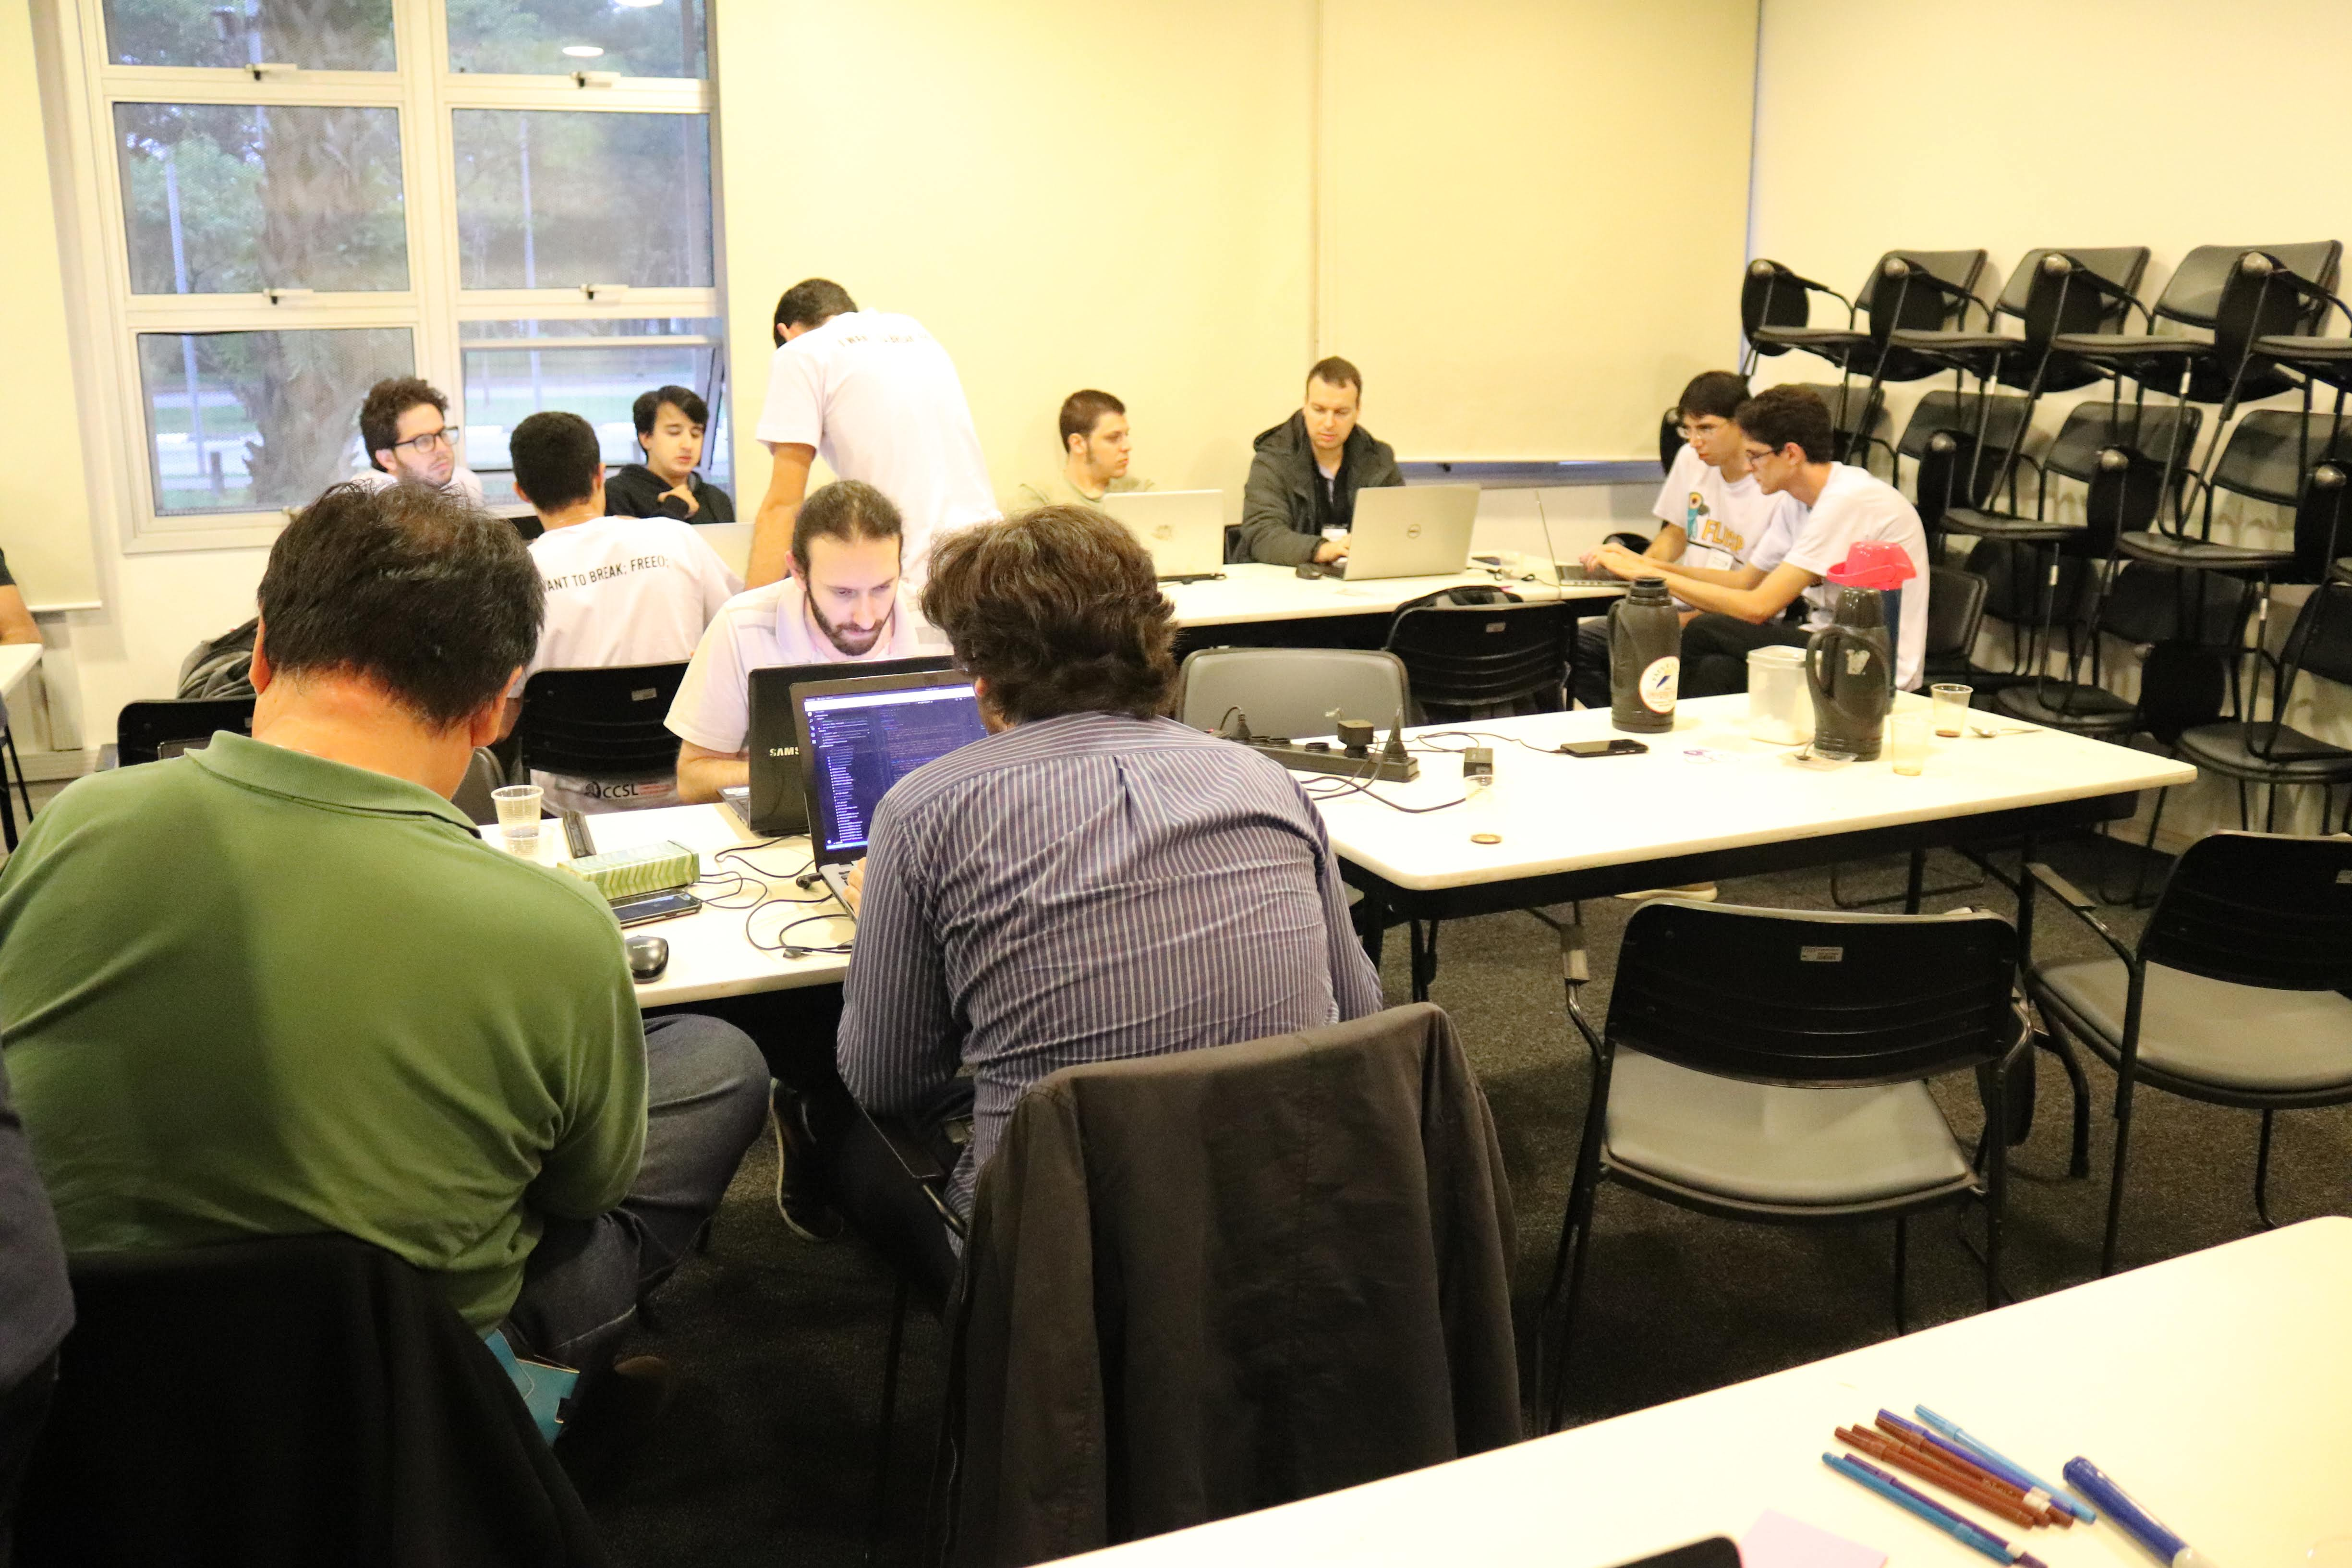
\includegraphics[height=0.4\paperheight]{afternoon1.jpg}
  \end{subfigure}
\end{figure}

\end{frame}

\begin{frame}{Overview}
  \overview
\end{frame}

\section{Introduction}


\begin{frame}{Introduction}
    \begin{itemize}
        \item How many of you have seen a compiler {\color{blue}{running in parallel}}?
    \end{itemize}
\end{frame}

\begin{frame}{Introduction}
    \begin{itemize}
        \item Parallelization of GCC Internals
        \begin{itemize}
            \item Without modifying the program compilation structure
            \item Exploring parallelism in a single file
        \end{itemize}
        \item[]
        \item Main objectives
        \begin{itemize}
            \item Reduction of compilation time
            \item Highlight GCC global states
        \end{itemize}
    \end{itemize}
\end{frame}

\begin{frame}{Motivation}
  \begin{itemize}
    \item Compilers are really complex programs
        \begin{itemize}
            \item GCC dates from 1987
            \item Still sequential
        \end{itemize}
    \item Automatic Generation of big files
        \begin{itemize}
            \item \texttt{gimple-match.c}: {\color{red}{100358 lines}} of C++ (GCC 10.0.0)
        \end{itemize}
    \item {\color{red}{Exponencial}} growth in {\color{blue}{number of cores}} of a CPU
  \end{itemize}
\end{frame}

\begin{frame}{Motivation}
    Growth of Computational Power \citep{42years}

    \centering
    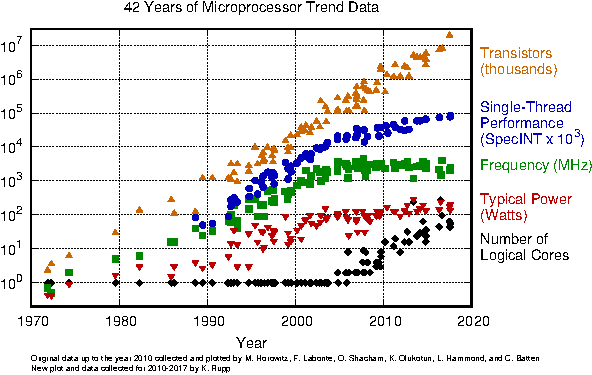
\includegraphics[scale=1.0]{42-years-processor-trend.pdf}
    \label{fig:42years}
\end{frame}


\begin{frame}{Motivation}
  \begin{itemize}
    \item Where can we use these parallel processors in a compiler?
    \item []
    \item How much the improvement is?
    \item []
    \item Is there projects that can be benefited from this?
  \end{itemize}
\end{frame}


\begin{frame}{Introduction}
    \begin{itemize}
        \item Experiment 1
        \begin{itemize}
            \item GCC compilation on a machine with $4\times$ AMD Opteron 6376
                \begin{itemize}
                    \item $4 \times 16 = 64$ cores
                \end{itemize}
            \item No \textit{bootstrap} (\texttt{--disable-bootstrap})
            \item Collected {\color{blue}{Compilation Time}} of {\color{red}{each file}}
            \item Collected {\color{blue}{Consumed Energy}} of {\color{red}{all CPUs}}
        \end{itemize}
    \end{itemize}
\end{frame}

\begin{frame}
    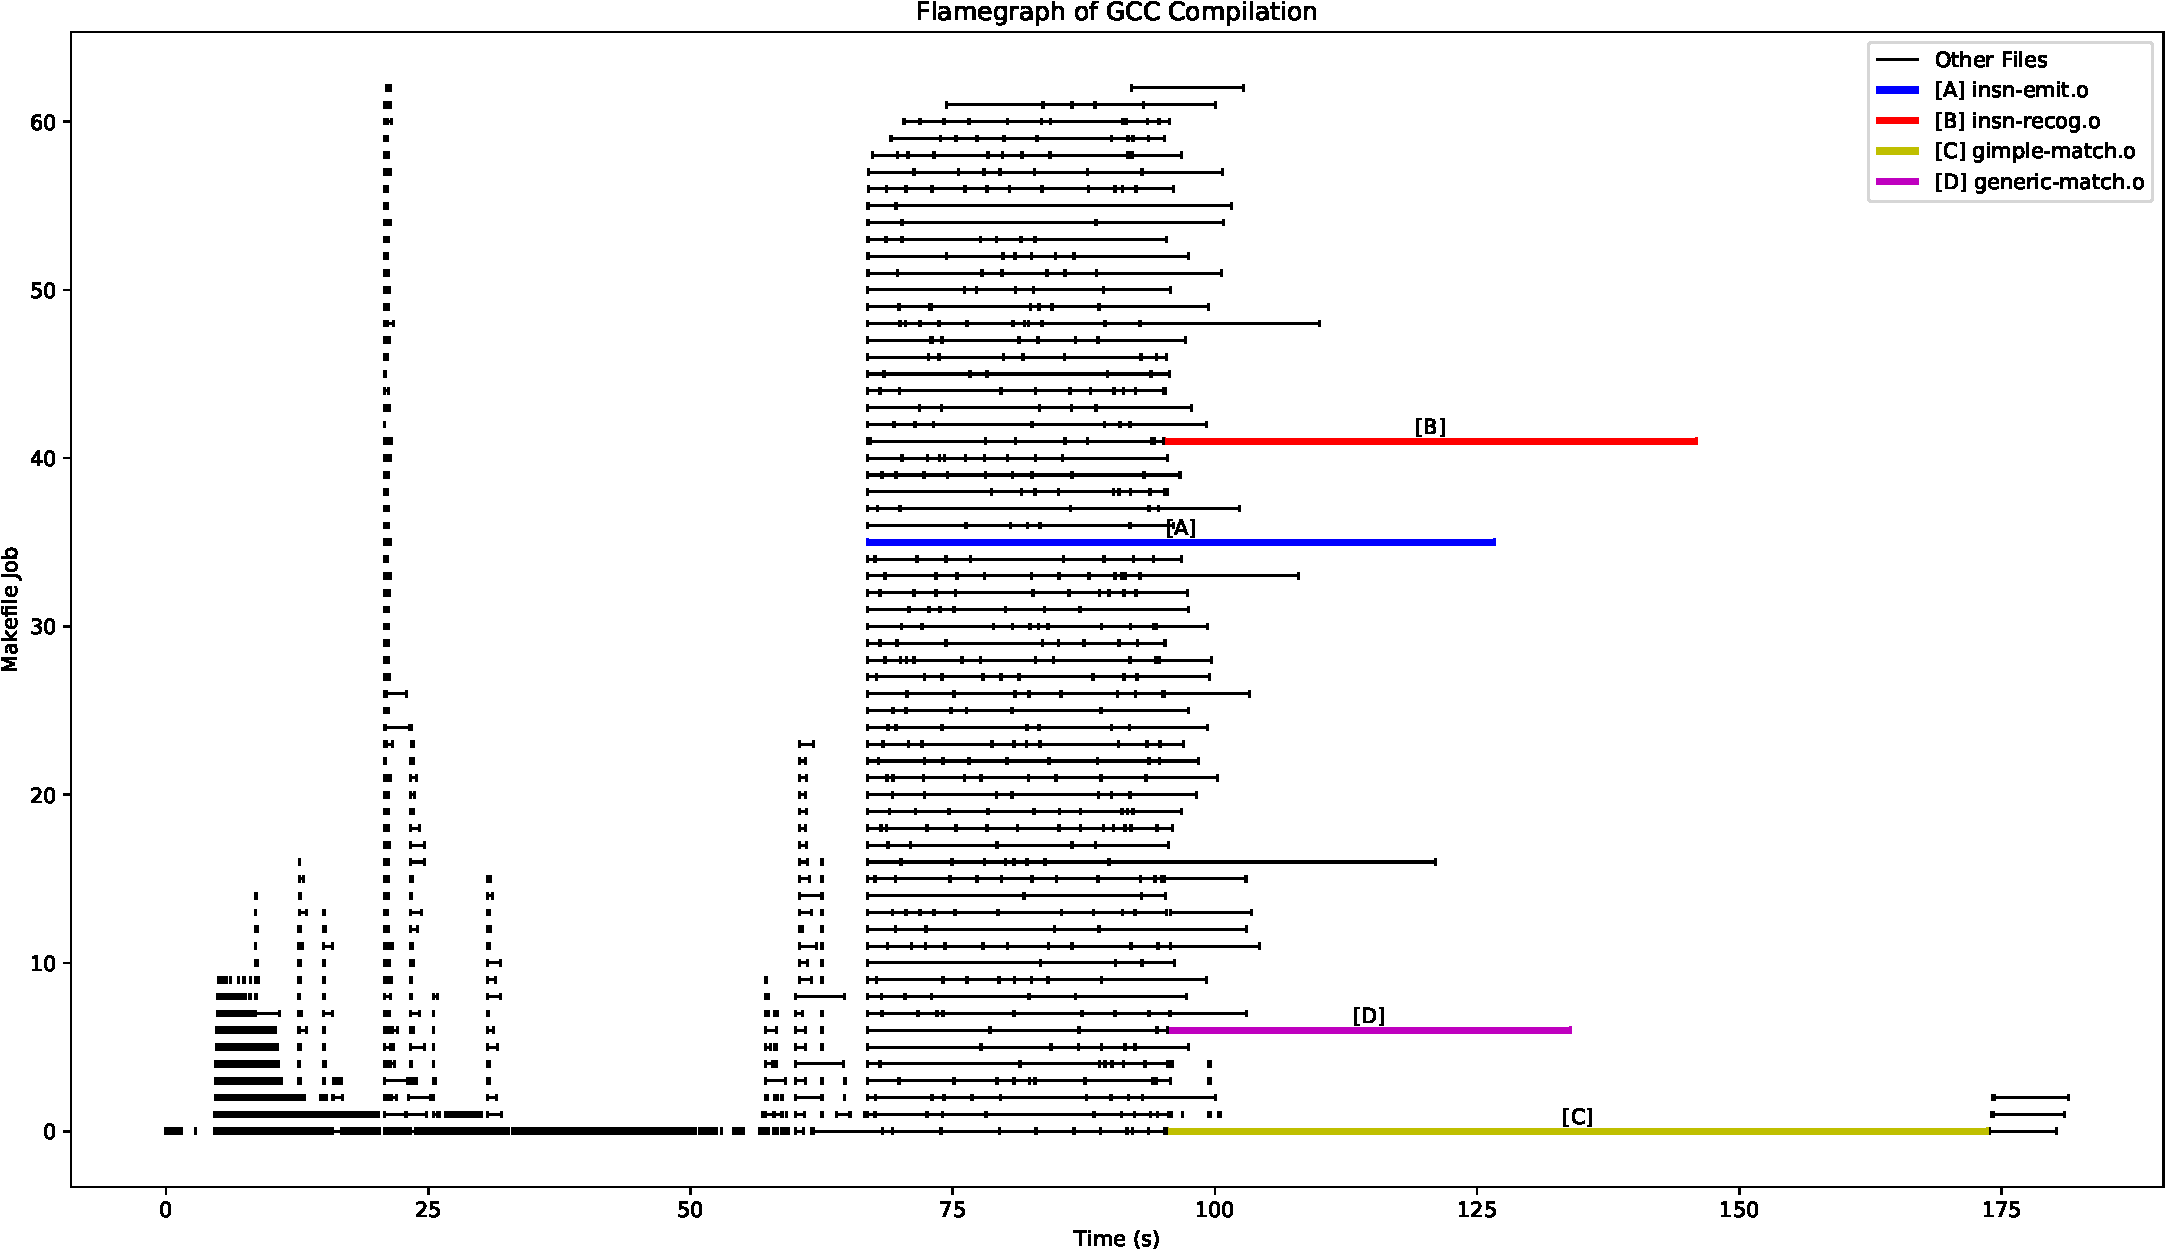
\includegraphics[width=0.9\paperwidth]{flamegraph.pdf}
    %   \captionof{figure}{Tempo corrido na compilação do GCC em um processador de
    %64 núcleos. \textbf{Sem} LTO, sem \textit{Bootstrap}.}
    \label{fig:analysis_classical}
\end{frame}

\begin{frame}
    \centering
    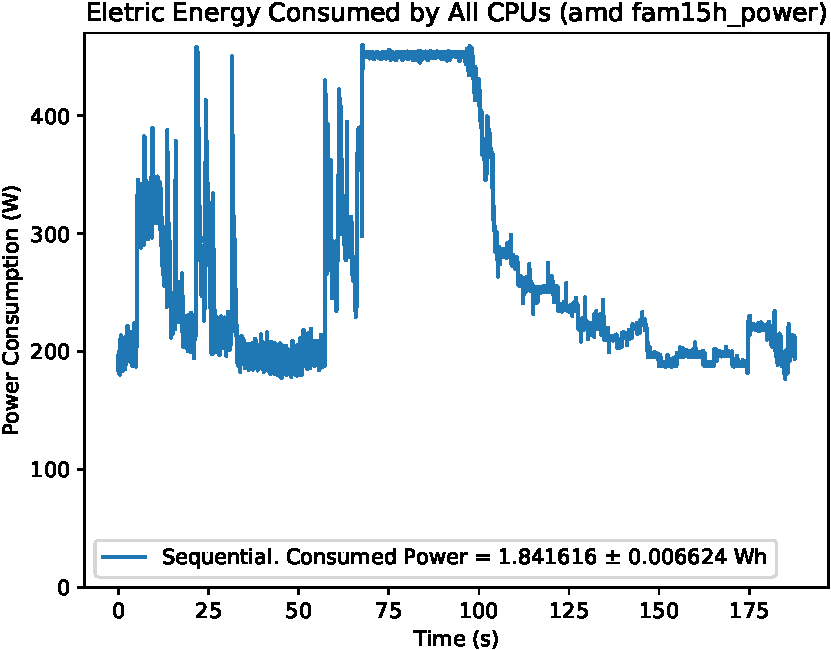
\includegraphics[height=0.8\paperheight]{sensor_graphic.pdf}
    %   \captionof{figure}{Tempo corrido na compilação do GCC em um processador de
    %64 núcleos. \textbf{Sem} LTO, sem \textit{Bootstrap}.}
    \label{fig:sensor_graphic}
\end{frame}


\begin{frame}{Introduction}
    \begin{itemize}
        \item How about LTO?
        \item[]
        \item Experiment 2
        \begin{itemize}
            \item GCC compilation on a machine with $4\times$ AMD Opteron 6376
                \begin{itemize}
                    \item $4 \times 16 = 64$ cores
                \end{itemize}
            \item No \textit{bootstrap} (\texttt{--disable-bootstrap})
            \item Enabled LTO (\texttt{CFLAGS=-flto=64 CXXFLAGS=-flto=64})
            \item Collected {\color{blue}{Compilation Time}} of {\color{red}{each file}}
            \item Collected {\color{blue}{Consumed Energy}} of {\color{red}{all CPUs}}
        \end{itemize}
    \end{itemize}
\end{frame}

\begin{frame}
    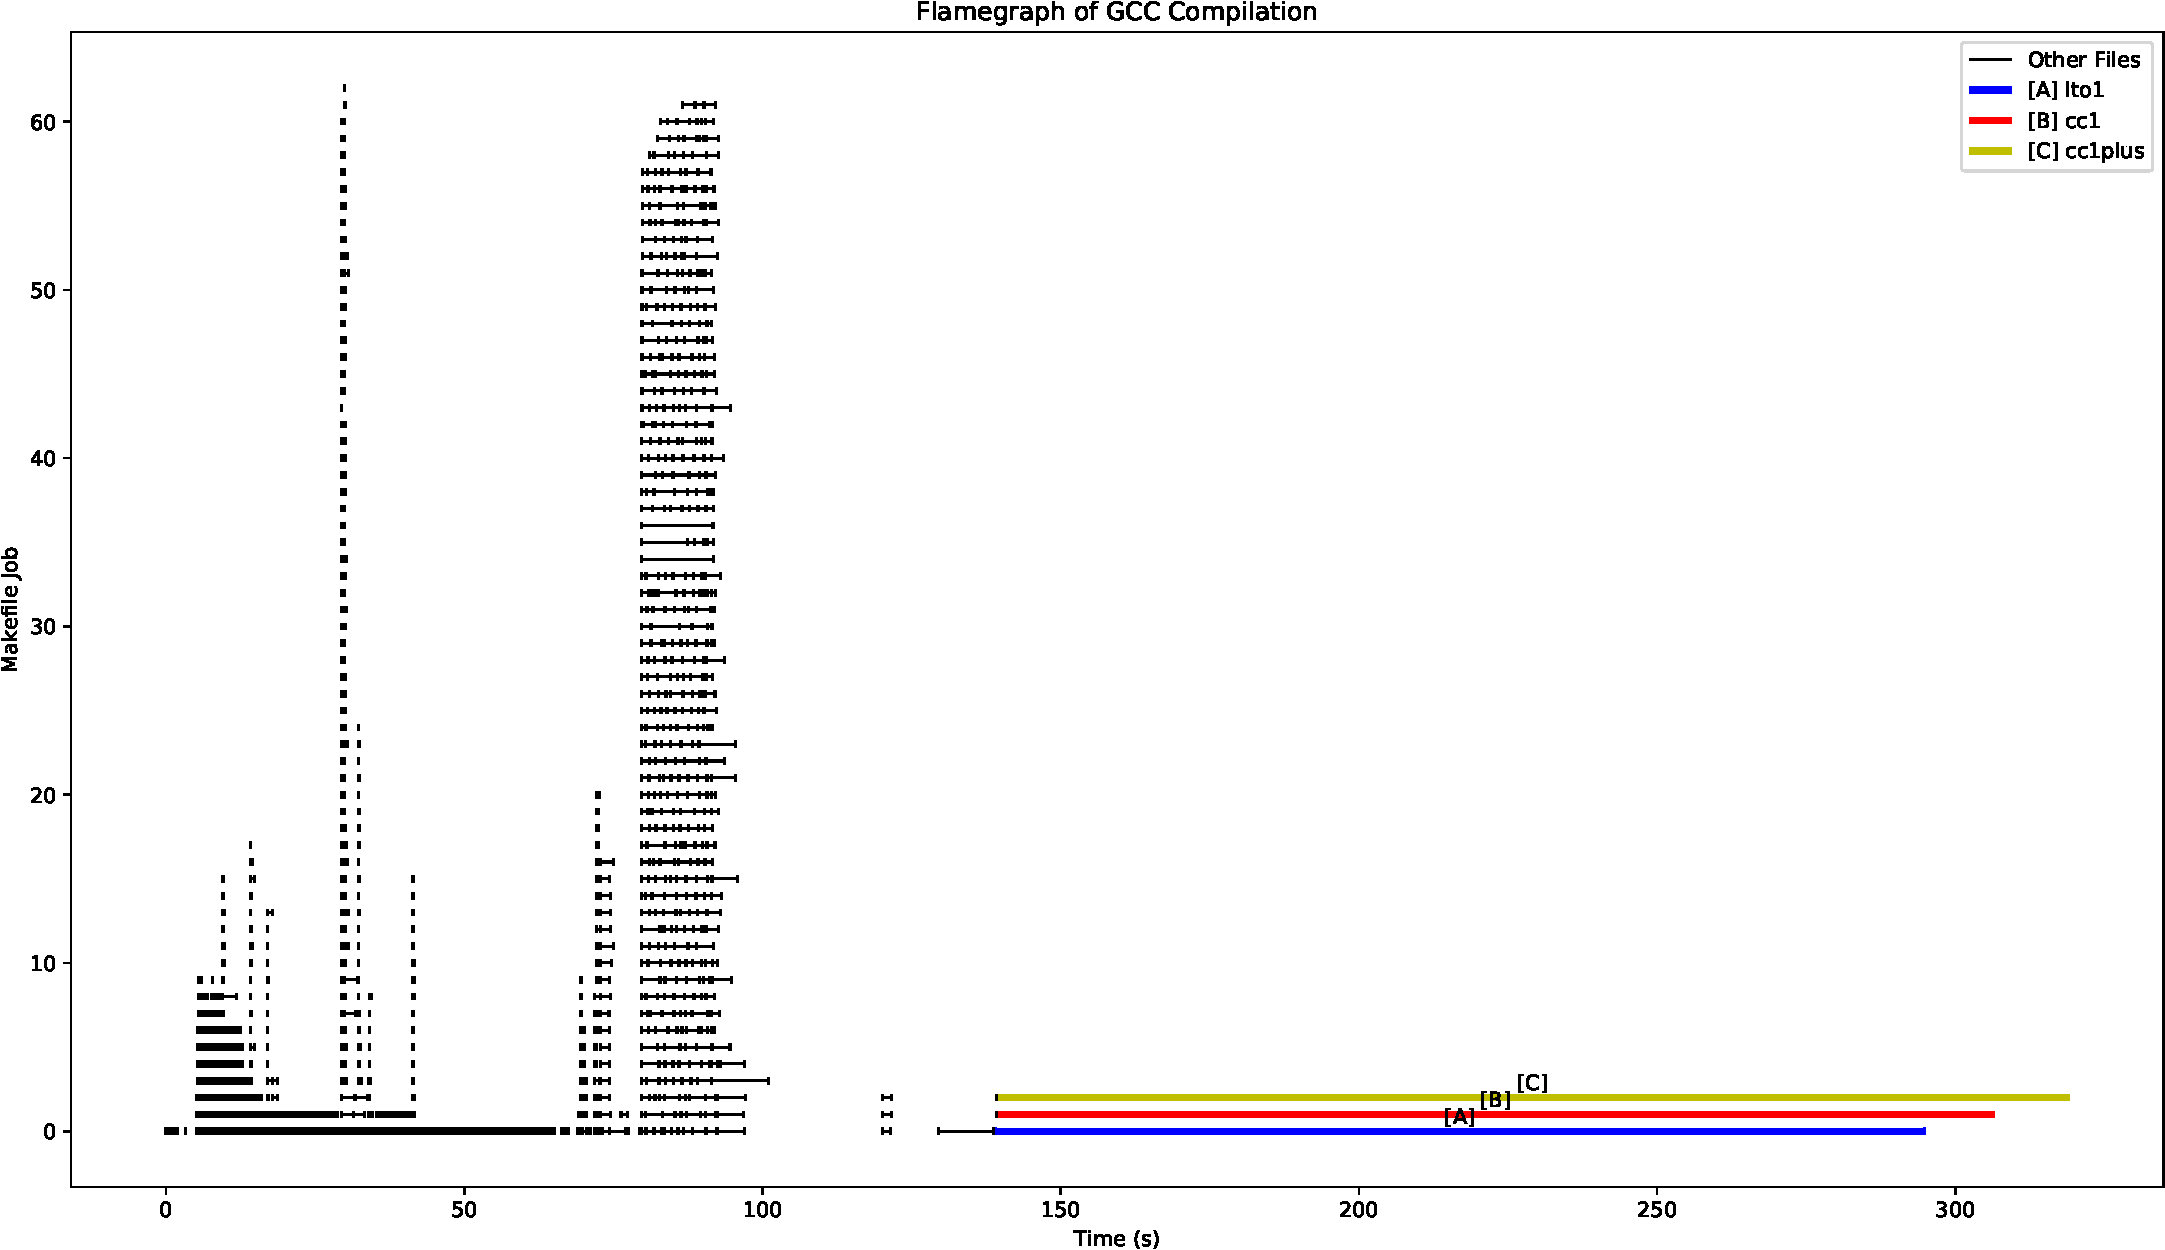
\includegraphics[width=0.9\paperwidth]{flamegraph_lto.pdf}
    %   \captionof{figure}{Tempo corrido na compilação do GCC em um processador de
    %64 núcleos. \textbf{Sem} LTO, sem \textit{Bootstrap}.}
    \label{fig:analysis_lto}
\end{frame}

\begin{frame}
    \centering
    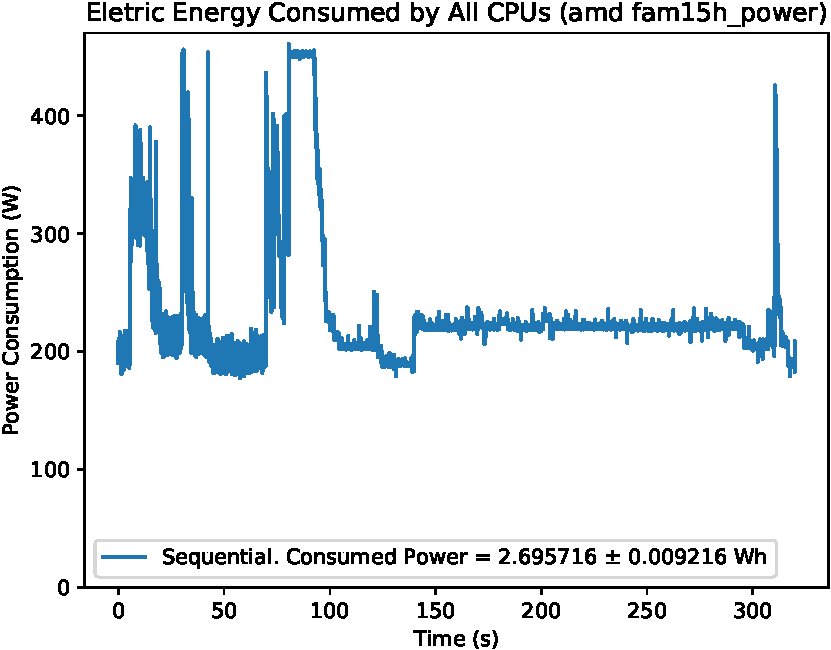
\includegraphics[height=0.8\paperheight]{sensor_graphic_with_lto.pdf}
    %   \captionof{figure}{Tempo corrido na compilação do GCC em um processador de
    %64 núcleos. \textbf{Sem} LTO, sem \textit{Bootstrap}.}
    \label{fig:sensor_graphic_lto}
\end{frame}


\begin{frame}{Results}
    \begin{itemize}
        \item There is a parallelism bottleneck in GCC project
        \item[]
        \item Could we improve it by parallelizing GCC?
    \end{itemize}
\end{frame}

\section{Where to Start?}

\begin{frame}{Where to Start?}
  GCC structure is divided in three parts.
  \begin{itemize}
    \item \textit{Front End}
        \begin{itemize}
            \item Parsing
        \end{itemize}
    \item \textit{Middle End}
        \begin{itemize}
            \item Hardware-Independent Optimization
        \end{itemize}
    \item \textit{Back End}
        \begin{itemize}
            \item Hardware-Dependent Optimization
            \item Code Generation
        \end{itemize}
  \end{itemize}
\end{frame}

\begin{frame}{Where to Start?}
  \begin{itemize}
    \item Selected Part: {\color{blue}{Middle End}}
    \begin{itemize}
        \item Applies Hardware-{\color{blue}{Independent}} Optimizations in the code
        \item Why? Because it was easier to start with rather than RTL
    \end{itemize}
    \item[]
    \item Optimization can be broken into two {\color{red}{disjoint}} sets
        \begin{itemize}
            \item {\color{blue}{Intra Procedural}}
                \begin{itemize}
                    \item Can be applied into a function without observing the interactions with other functions
                \end{itemize}
            \item {\color{red}{Inter Procedural}}
                \begin{itemize}
                    \item Interaction with other functions must be considered
                    \item GCC calls this Inter Process Analysis (IPA)
                \end{itemize}
        \end{itemize}
  \end{itemize}
\end{frame}

\begin{frame}{GCC Profile}
    \begin{itemize}
        \item We used \texttt{gimple-match.c} to profile the compiler
            \begin{itemize}
                \item Intel Core i5-8250U (4 cores)
                \item 5400RPM 1TB Hard Drive
            \end{itemize}
    \end{itemize}

            \centering
            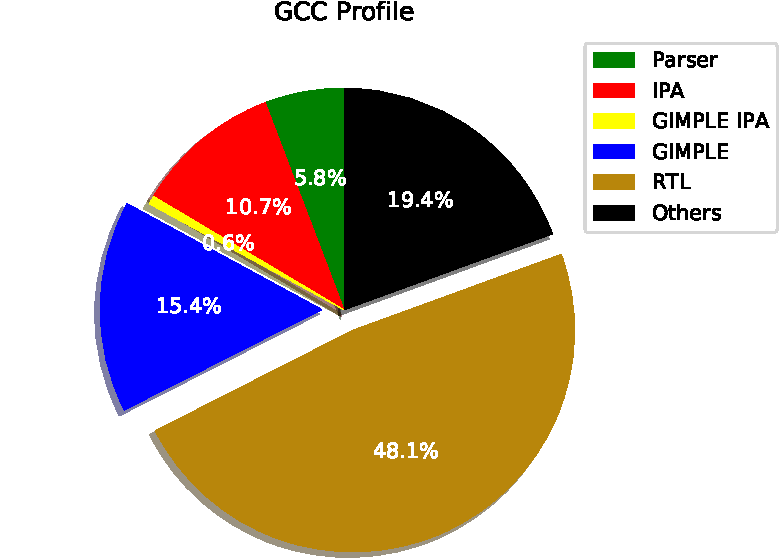
\includegraphics[scale=0.5]{profile_pie.pdf}
\end{frame}

\begin{frame}{GCC Profile}
    \begin{itemize}
        \item We used \texttt{gimple-match.c} to profile the compiler
            \begin{itemize}
                \item 63\% is spent in Intra Procedural Optimization
                \item This can be parallelized
                \item Maximum speedup: $2.7\times$ according to Amdahl's Law
            \end{itemize}
    \end{itemize}

\end{frame}

\section{Parallel Approach}

\begin{frame}{Parallel Approach}
    \begin{itemize}
        \item Parallelize Intra Procedural Optimizations
            \begin{itemize}
                \item By per-function
                \item Similarly to \cite{wortman1992}
                \item With arbitrary number of threads
    \end{itemize}
\end{itemize}

\end{frame}

\begin{frame}{Parallel Approach}
    \begin{itemize}
        \item Parallel Architecture of the Compiler
            \begin{itemize}
                \item The Inter Process Analysis inserts functions into a Producer Consumer Queue
                \item Each thread is responsible to remove their work from the Queue
                \item When Queue is empty, threads are blocked until work is inserted into it
                \item The threads die when the \texttt{EMPTY} token is inserted
                \item Measured overhead: 0.1s for 2000 functions
             \end{itemize}
\end{itemize}
 \centering
 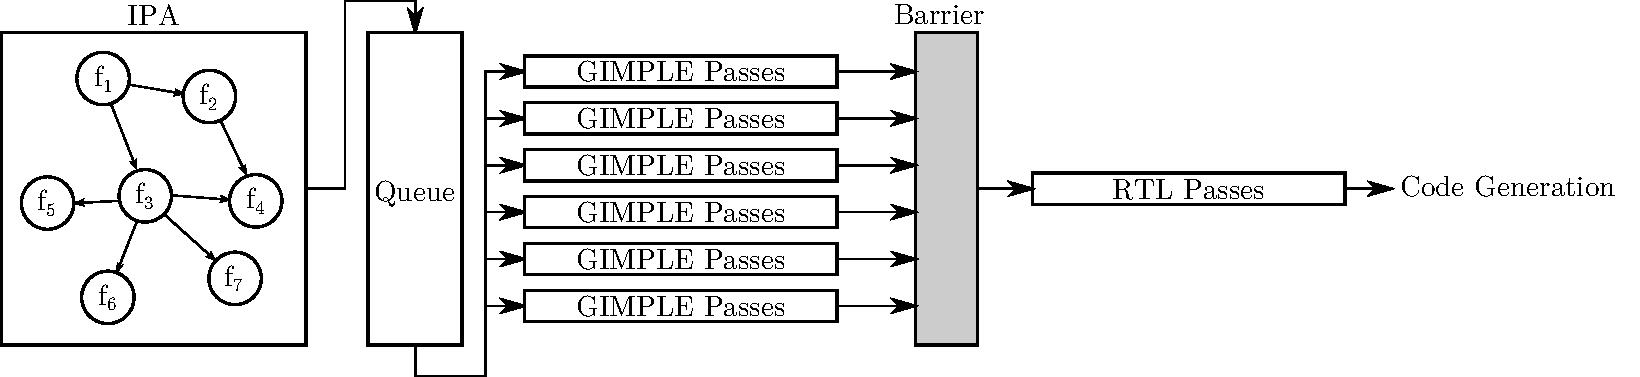
\includegraphics[width=\textwidth]{paralelizacao_eng.pdf}
\end{frame}

\begin{frame}{Parallel Approach}
    \begin{itemize}
        \item Advantages
            \begin{itemize}
                \item Best candidate to Linear speedup
                \item Worst case: A single big function
            \end{itemize}
        \item Disadvantage
            \begin{itemize}
              \item Map per-pass global states in the compiler
            \end{itemize}
    \end{itemize}
\end{frame}

\begin{frame}{Implementation}
    \begin{itemize}
        \item Split \texttt{cgraph\_node::expand} into three methods:
            \begin{enumerate}
                \item \texttt{expand\_ipa\_gimple}
                \item \texttt{expand\_gimple} $\longleftarrow$ Parallelization effort in GSoC 2019
                \item \texttt{expand\_rtl}
            \end{enumerate}
        \item Serialized the Garbage Collector
        \item Serialized memory related structures
    \end{itemize}
\end{frame}

\begin{frame}{Implementation}
    Memory Pools:
    \begin{itemize}
        \item Problems:
            \begin{itemize}
                \item Linked List of several object instances
                \item Can be allocated/released upon request
                \item Most race conditions were there
            \end{itemize}
        \item Solution:
            \begin{itemize}
                \item Create an instance for every thread
                \item Merge the memory pools when all threads join
                \item Implementing merge feature: Just append the two Linked List
            \end{itemize}
    \end{itemize}
\end{frame}

\begin{frame}{Implementation}
    Garbage Collection: 
    \begin{itemize}
        \item Problem: 
            \begin{itemize}
                \item GCC implements a garbage collector 
                \item Variables can be marked to be watched by it
                \item Collection can also be done upon request
            \end{itemize}
        \item Partial Solution:
            \begin{itemize}
                \item Serialize the entire Garbage Collector
                \item Disable collection between passes
            \end{itemize}
        \item Research is needed to:
            \begin{itemize}
                \item Map the race conditions in the Garbage Collector 
                \item Make it thread aware
            \end{itemize}
    \end{itemize}
\end{frame}

\begin{frame}{Implementation}
    \texttt{rtl\_data} Structure: 
    \begin{itemize}
        \item Problem: 
            \begin{itemize}
                \item This class represents the current function being compiled in RTL
                \item GCC only has a single instance of this class
                \item GIMPLE uses it to decide optimization related to instruction costs
            \end{itemize}
        \item Partial Solution:
            \begin{itemize}
                \item Have one copy of this structure for each thread 
            \end{itemize}
        \item Solution 
            \begin{itemize}
                \item Do not rely on it at this stage of compilation? 
            \end{itemize}
    \end{itemize}
\end{frame}

\begin{frame}{Implementation}
    tree-ssa.address.c: \texttt{mem\_addr\_template\_list} 

    \begin{itemize}
        \item Problem:
            \begin{itemize}
                \item Race condition in this structure
            \end{itemize}
        \item Partial Solution:
            \begin{itemize}
                \item Serialize with a mutex
            \end{itemize}
        \item Solution 
            \begin{itemize}
                \item Replicate for each thread?
            \end{itemize}
    \end{itemize}

\end{frame}

\begin{frame}{Implementation}
    Integer to Tree Node hash

    \begin{itemize}
        \item Problem:
            \begin{itemize}
                \item Race condition in this structure
            \end{itemize}
        \item Partial Solution:
            \begin{itemize}
                \item Serialize with a mutex
            \end{itemize}
        \item Solution 
            \begin{itemize}
                \item Replicate for each thread?
            \end{itemize}
    \end{itemize}
\end{frame}


\section{Results}

\begin{frame}{Results}
    \begin{itemize}
        \item Results by parallelizing GIMPLE
        \item Mean of 30 samples
    \end{itemize}

\begin{figure}[ht]
\centering
  \begin{subfigure}[b]{0.49\textwidth}
 	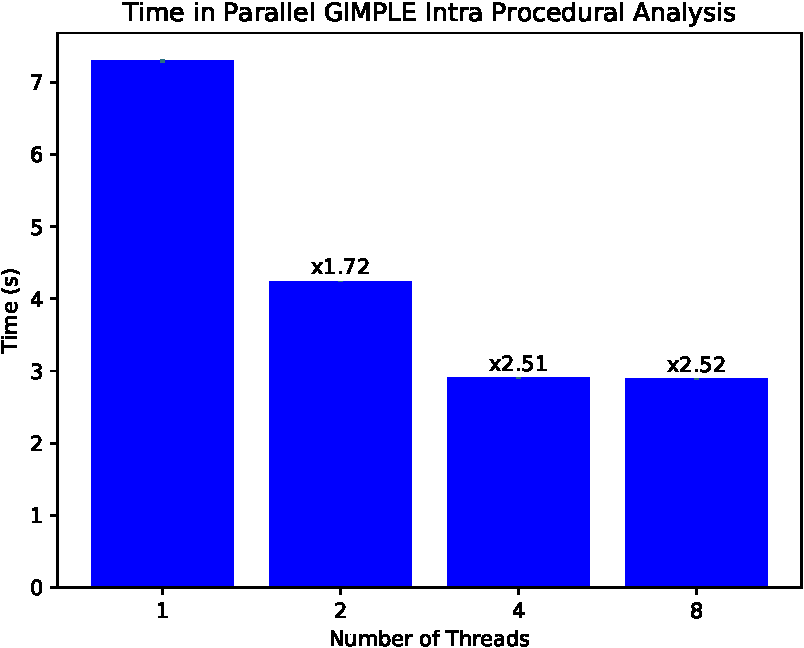
\includegraphics[scale=0.45]{gimple_speedup.pdf}
  \end{subfigure}
  \begin{subfigure}[b]{0.49\textwidth}
 	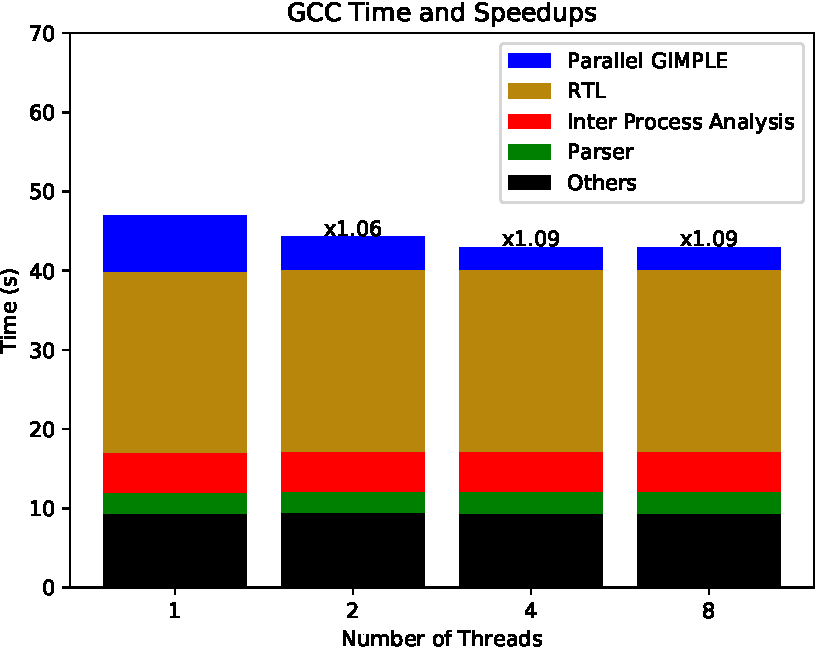
\includegraphics[scale=0.45]{gcc_archived_speedup.pdf}
  \end{subfigure}
\end{figure}
\end{frame}

\begin{frame}{Results}
    \begin{itemize}
        \item The same approach can be used to parallelize RTL
        \item Using the GIMPLE results
    \end{itemize}

\begin{figure}[ht]
\centering
 	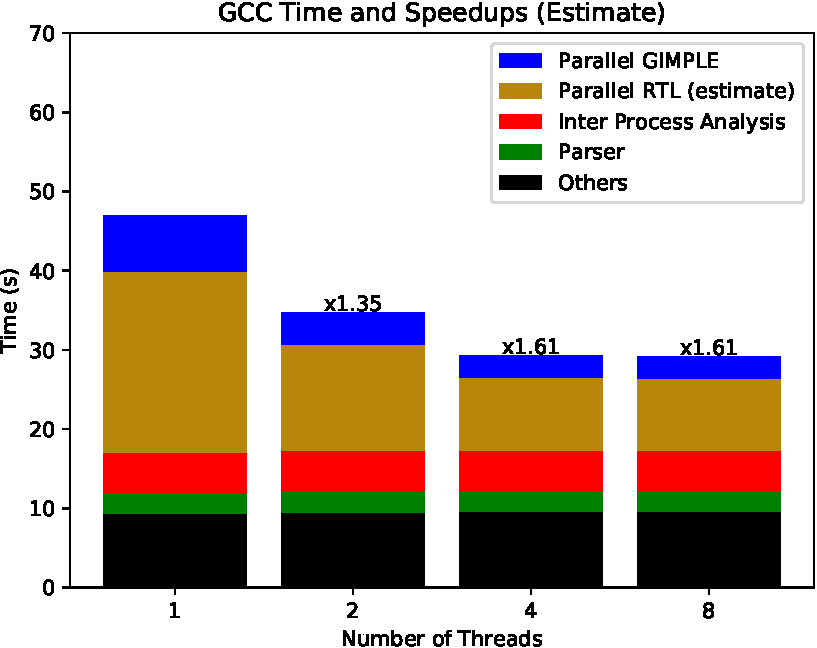
\includegraphics[scale=0.5]{gcc_estimate.pdf}
\end{figure}
\end{frame}



\begin{frame}{Motivation}
  \begin{itemize}
    \item Where can we use these parallel processors in a compiler?
        \begin{itemize}
            \item Intra Process Analysis is a easy answer
        \end{itemize}
    \item []
    \item How much the improvement is?
        \begin{itemize}
            \item Without much optimization, $1.6\times$ using 4 threads
            \item Better results will require more effort
        \end{itemize}

    \item []
    \item Is there projects that can be benefited from this?
        \begin{itemize}
            \item GCC
        \end{itemize}
  \end{itemize}
\end{frame}

\section{TODOs}

\begin{frame}{TODOs}
    \begin{itemize}
        \item What is left to do:
            \begin{itemize}
                \item Fix all race conditions in GIMPLE
                \item Fix all C11 \texttt{\_\_thread} occurrences
                    \begin{itemize}
                        \item Initialize Inter-Pass objects at \texttt{::execute} time
                        \item Per-thread attributes initialized at spawn time
                    \end{itemize}
                \item Parallelize RTL
                \item Parallelize IPA (useful for LTO?)
                \item Communicate with Make for automatic threading
            \end{itemize}
    \end{itemize}
\end{frame}

%\section{Metodologia de Validação}
%
%\begin{frame}{Metodologia de Validação}
%    \begin{itemize}
%        \item Técnicas de inferência estatística medição de tempo
%            \begin{itemize}
%                \item Distribuição Probabilística do tempo de compilação
%                \item Teorema do Limite Central
%                \item Intervalos de Confiança
%            \end{itemize}
%        \item Técnica para verificação de corretude
%            \begin{itemize}
%                \item Execução dos 62180 testes do GCC
%                \item \textit{Bootstrap} (compilar a si mesmo)
%            \end{itemize}
%        \item Técnica para cálculo de Energia Consumida
%        \begin{itemize}
%            \item Uso do sensor \texttt{amd fam15h\_power}
%            \begin{itemize}
%                \item Mede a potência instantânea enviada à CPU pela \textit{Northbridge}
%            \end{itemize}
%
%            \item Definição de Potência Instantânea
%            \item Integral numérica
%            \item Teorema do Confronto
%        \end{itemize}
%    \end{itemize}
%\end{frame}

\section{References}

\begin{frame}[allowframebreaks]{References}
  %\nocite{bronevetsky02, schmidt03:MSc, FSF:GNU-GPL, CORBA:spec, MenaChalco08, natbib, biblatex, eco:09}
  \printbibliography
\end{frame}

% Recapitulando
\begin{frame}{Repositories}
  \overview

  % \begin{center} acrescenta espaço vertical;
  % como possivelmente temos bem pouco espaço aqui,
  % vamos usar centering
  {%
    \centering\noindent%
    \url{https://github.com/giulianobelinassi/gcc-timer-analysis}\par
    \url{https://gitlab.com/flusp/gcc/tree/giulianob\_parallel}\par
    \url{https://gcc.gnu.org/wiki/ParallelGcc}\par
  }

\end{frame}

\begin{frame}[standout]
    Thank you!
\end{frame}

\appendix

